% 第6章 本研究の詳細
\newpage
\renewcommand{\baselinestretch}{1.5}
\section{本研究の詳細}
\renewcommand{\baselinestretch}{1}

\par デザイナーが検証するウェブページのURLを入力すると該当ページの顕著性マップとページの構造を組み合わせることにより顕著度が高い領域を要素単位で分析して顕著領域マップを出力する手法を提案する。また、一般ユーザー向けに特に顕著度が高い領域を纏めて描写した集約図を出力する手法を提案する。本手法の構造図を図\ref{fig_ourmodel}に示す。

\begin{figure}[H]
    \centering
    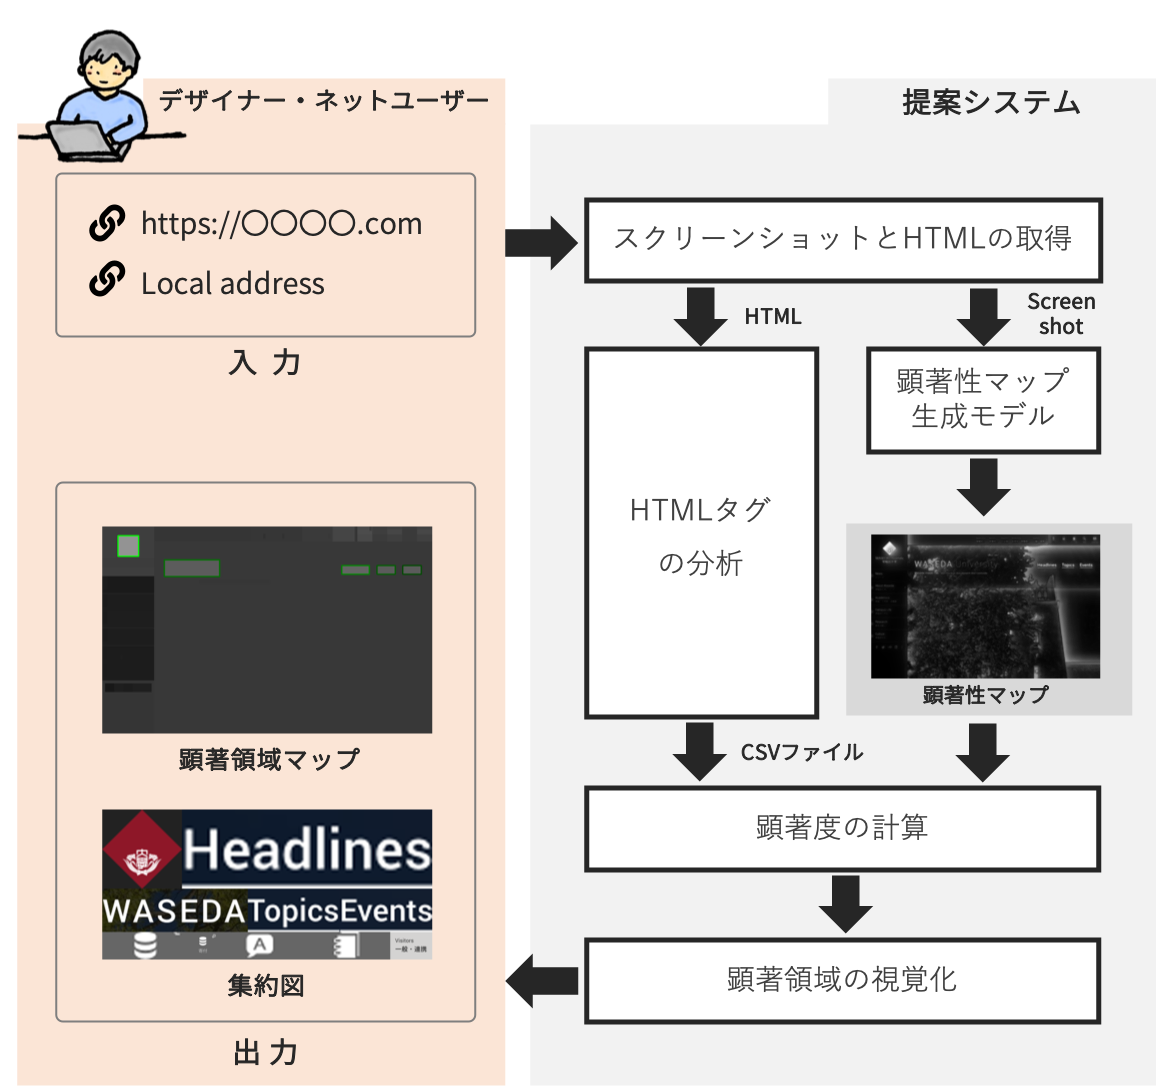
\includegraphics[width=9cm]{figures/model.png}
    \caption{モデルの図}
    \label{fig_ourmodel}
\end{figure}

\par 本手法の手順は以下の通りである。
\par(1) HTMLの取得と顕著性マップの生成
\par(2) HTMLの解析によるタグの分析と位置の取得
\par(3) 顕著度の計算
\par(4) 顕著領域の視覚化\\

\par なお、本研究ではウェブスクレイピング技術としてSelenium WebDriverとBeautiful Soupを使用するが別のスクレイピング技術を使用しても実装は可能である。また、スクリーンショットを取得するブラウザとしてFirefoxを使用するがChromeなど別のブラウザでも実装可能である。

\subsection{HTMLの取得と顕著性マップの生成}\label{subsec:system01}
% ウェブスクレイピング技術を使用してスクショを取得する方法とHTMLの取得方法の記述
% スクショのグレースケール変換方法・サイズの圧縮
%  Selenium WebdriverでFirefoxの立ち上げ・該当URLへの移動
%  Selenium WebdriverでHTMLの取得
%  Beautiful Soupを用いてHTMLの整形
%  Selenium Webdriverでスクショの取得・保存
%  顕著性マップの生成
%  OpenCVを用いて顕著性マップの二値化  
%  OpenCVを用いてスクショと顕著性マップの指定サイズへの圧縮

\par 本システムではまず、入力されたURL情報を元に\ref{sec:scraping}で説明したウェブスクレイピング技術を用いてスクリーンショットとHTMLを取得する。また、取得したスクリーンショットを用いて顕著性マップを生成する。デザイナーが開発段階で簡単に使用可能な様に入力するURLは、ネットワーク上に存在するウェブページだけでなくローカル環境のURLにも対応させている。HTMLの取得と顕著性マップの生成の流れを図\ref{fig_system01}に示す。

\begin{figure}[H]
    \centering
    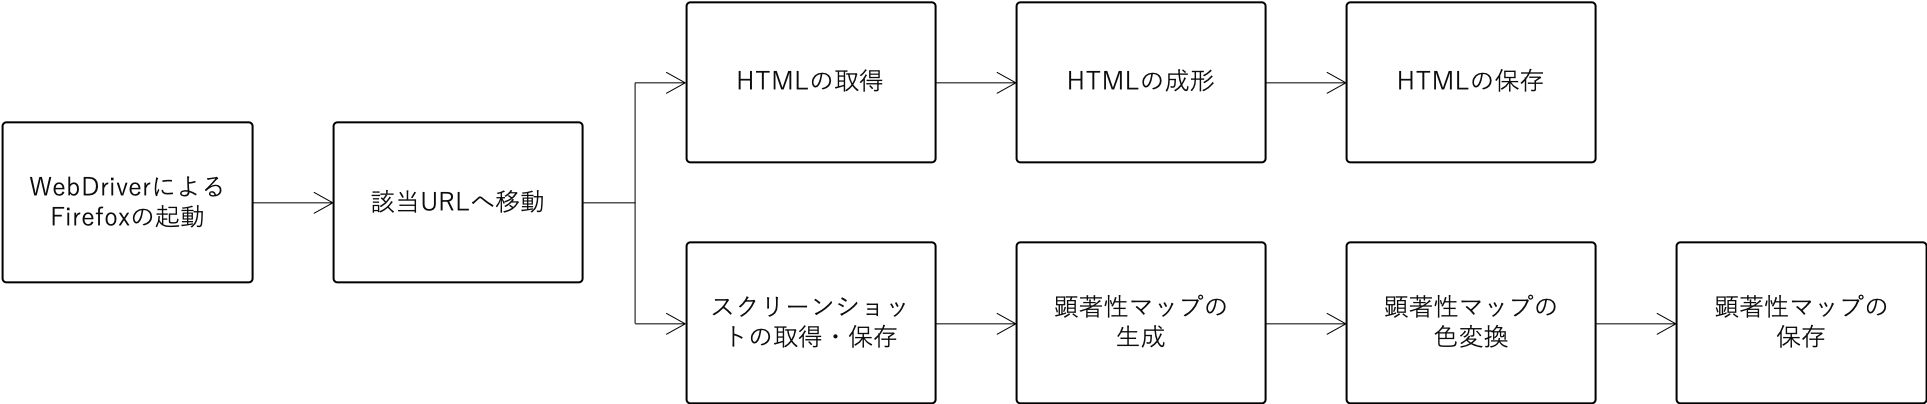
\includegraphics[width=12cm]{figures/system01.png}
    \caption{HTMLの取得と顕著性マップの生成の流れ}
    \label{fig_system01}
\end{figure}

\par まず始めに、Selenium WebDriverを用いてFirefoxを起動し、ブラウザのウィンドウサイズを一般的なパソコンで閲覧する条件に近い横1280px縦900pxに設定する。次に入力されたURLにアクセスを行い、ウェブページの読み込みが完了したらHTMLの取得を行う。取得したHTMLはインデントなどが乱れた状態である為、Selenium WebDriverと同じくウェブスクレイピング技術のライブラリであるBeautiful Soup\cite{beautifulsoup}を使用して扱いやすい状態に整形を行った後に保存する。

\par 次にウェブページのスクリーンショットを取得する。取得するスクリーンショットは、重要度が高いコンテンツはウェブページの最上部に存在する可能性が高いという考えから、ウェブページにアクセスした時点で閲覧可能な最上部の横1280px縦900pxとした。さらに、取得したスクリーンショットから顕著性マップを生成する。顕著性マップの生成には第\ref{subsec:itti-kochi}節で説明したItti-Kochらの顕著性マップ生成モデルを使用した。本来であれば、ウェブページに最適化された精度の高いモデルを使用すべきであるが現時点では技術的に難しいと判断し扱いやすいモデルを使用することにした。ここで顕著性マップ生成モデルにより出力される顕著性マップはRGBの3色チャンネルで出力されるが、後の処理で明度を使用するために単色チャンネルで表されるグレースケール画像に変換して保存する。取得される顕著性マップの例が図\ref{fig_example-saliencymap}(右)である。


\subsection{HTMLの解析によるタグの分析と位置の取得}\label{subsec:system02}
% 各タグの存在確認と位置情報の取得方法の記述
%  CSVの準備(ヘッダーの準備)
%  Selenium Webdriverで各タグの位置情報の取得(xpathとサイズ取得方法の説明を入れる)

\par ここでは第\ref{subsec:system01}節で取得したHTMLの解析を行いウェブページ上の要素の位置情報とそのサイズを取得する。HTMLの解析によるタグの分析と位置の取得の流れを図\ref{fig_system02}に示す。

\begin{figure}[H]
    \centering
    
\includegraphics[width=12cm]{figures/system02.png}
    \caption{HTMLの解析によるタグの分析と位置の取得の流れ}
    \label{fig_system02}
\end{figure}

% 左上を(0,0)として、、みたいなことを記述しないとわからない!!!!
\par まず始めに第\ref{subsec:system01}節で取得したHTMLの分析を行い、Selenium WebDriverで表\ref{table:gettaglist}に示す7個のタグ要素のidまたはclass名と左上の頂点の座標と縦と横のサイズを取得した後にCSVファイルに書き出す。座標の取得箇所を図\ref{fig_getposition}に示す。ウェブブラウザの左上を基準点(0,0)として基準点からの距離を要素の座標とした。また、時間短縮とエラーを防ぐために画面上に表示されている要素のみを取得する。なお、標準サイズのテキストを表すタグである\textless p\textgreater は通常、ウェブページの顕著度に大きく影響を与えないと判断したため取得しない。

\begin{table}[h]
    \caption{位置情報とサイズを取得するタグの一覧}
    \label{table:gettaglist}
    \centering
     \begin{tabular}{clll}
      \hline
      タグ & 意味 \\
      \hline \hline
      \textless div\textgreater & ブロック要素を表す \\
      \textless h1\textgreater & 文書中の見出しを示す為の要素で最も重要 \\
      \textless h2\textgreater & 文書中の見出しを示す為の要素で2番目に重要 \\
      \textless h3\textgreater & 文書中の見出しを示す為の要素で3番目に重要 \\
      \textless a\textgreater & リンクを示す \\
      \textless span\textgreater & インライン要素を示し、重要な要素が多い \\
      \textless img\textgreater & 画像要素を表す \\
      \hline
    \end{tabular}
\end{table}

\begin{figure}[H]
    \centering
    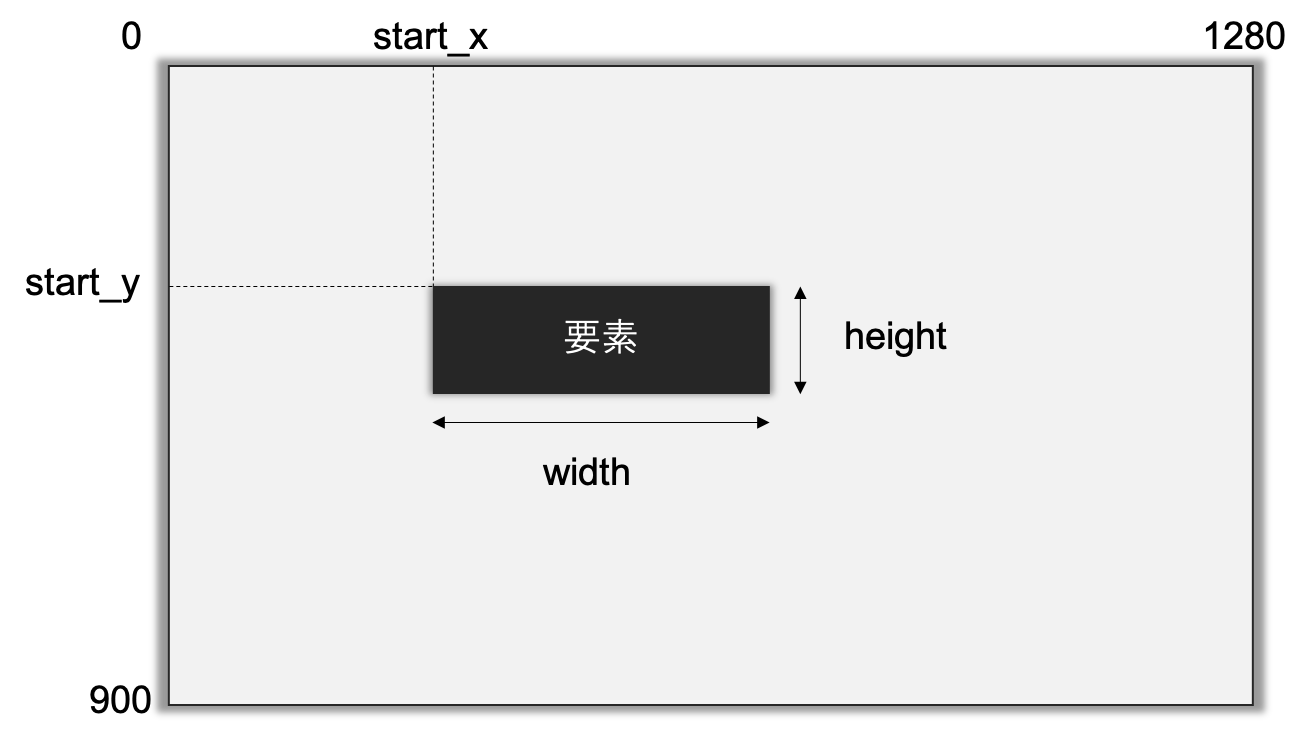
\includegraphics[width=8cm]{figures/getposition.png}
    \caption{基準点と要素の座標取得}
    \label{fig_getposition}
\end{figure}


\subsection{顕著度の計算}\label{subsec:system03}
% 領域のサイズ・位置による重み付けを行うことの記述・顕著度のランキングの取得方法
% F-bias Center-bias Webpage Saliencyより
% サイズによる重み付け
% 擬似プログラム
\par ここでは第\ref{subsec:system01}節で生成した顕著性マップと第\ref{subsec:system02}節で取得した各タグ要素の位置情報とサイズを比較して各要素の顕著度を計算する。顕著度の計算の流れを図\ref{fig_system03}に示す。

\begin{figure}[H]
    \centering
    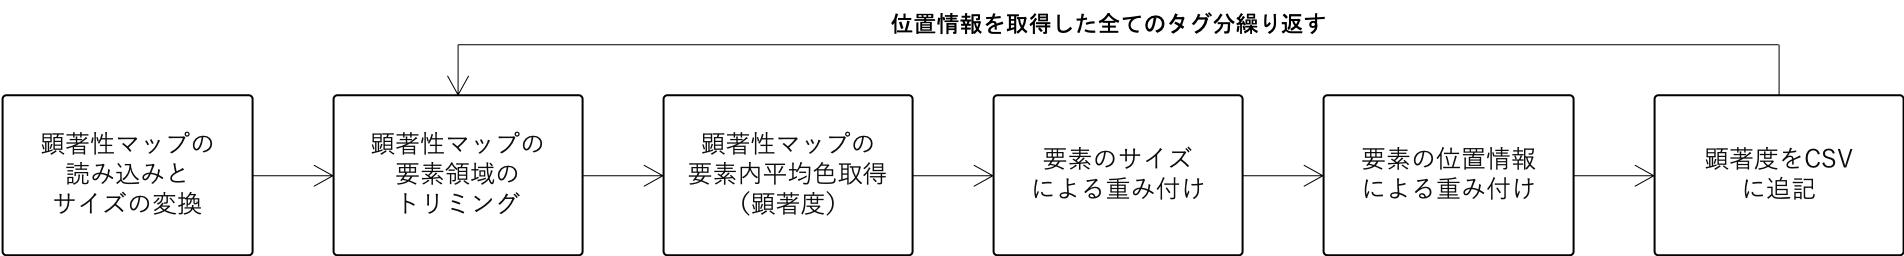
\includegraphics[width=12cm]{figures/system03.png}
    \caption{顕著度の計算の流れ}
    \label{fig_system03}
\end{figure}

\par まず始めに第\ref{subsec:system01}節で保存した顕著性マップを読み込む。使用端末により異なるが最近のパソコンは画面の高画質化が進み、横1280px縦900pxで撮影したスクリーンショットはその倍近い解像度で保存されている。その為、単純に顕著性マップを読み込み要素の位置情報と照らし合わせるとズレが生じてしまう。この問題を解決する為に読み込んだ顕著性マップを圧縮加工して取得した位置情報と同じサイズに合わせる必要がある。

\par 次に第\ref{subsec:system02}節で取得した各タグ要素毎に読み込んだ顕著性マップの該当要素の領域をトリミングする。また、トリミングした領域の色の明度の平均を計算する事で顕著度を計算する。しかしながら、単純に色の明度の平均を要素の顕著度にすると極端に小さな要素の顕著度が高く判定されてしまうなどの問題が生じた。そこで、本システムでは要素のサイズと位置による顕著度の重み付けを行う事でより正確に顕著度を判定出来るように工夫した。

\subsubsection{要素のサイズによる重み付け}\label{subsec:system03-1}
\par 先ほど述べた通り、単純に要素の明度の平均を取得すると小さな要素の顕著度が極端に高く計算される傾向があることが判明した為、要素の大きさによる重み付けを行うことで顕著度を平均化する。本来であれば深層学習等を用いて適切な重み付けを学習するのが良いが、本研究では実験を何度か行い極端に小さな要素の顕著度を低く判断する様に重み付けを独自の基準でアルゴリズム\ref{alg:weight-size}のように設定した。取得した要素の明度の平均値に重みをかける事で実装する。

\begin{algorithm}[H]
    \caption{サイズによる重み付け}
    \label{alg:weight-size}
    \begin{algorithmic}
    \Function{calc\_salient\_level}{start\_x, start\_y, size\_w, size\_h}
    \State salient\_level $ \leftarrow $ 要素の明度の平均値(0-255)
    \State salient\_level\_weight = size\_w * size\_h //要素の面積を計算
    \If{salient\_level\_weight $>$ 1000}
        \State salient\_level $ \leftarrow $ salient\_level
    \ElsIf{salient\_level\_weight $>$ 800}
        \State salient\_level $ \leftarrow $ salient\_level * 0.7
    \ElsIf{salient\_level\_weight $>$ 500}
        \State salient\_level $ \leftarrow $ salient\_level * 0.6
    \Else
        \State salient\_level $ \leftarrow $ salient\_level * 0.2
    \EndIf
    \State \Return salient\_level
    \EndFunction
    \end{algorithmic}
\end{algorithm}

\subsubsection{要素の位置による重み付け}\label{subsec:system03-1}
\par 関連研究でも触れたShenら\cite{shen2014webpage}の人間の目の視線を測定するアイトラッカーを用いてウェブページの顕著性を測定した実験によると、図\ref{fig_shen-experience}に示すようにテキスト中心と画像中心とテキスト画像が混合した全てのウェブページにおいて人は左上の領域と中心付近に目線が行く傾向が判明した。ウェブページの左上から中央にかけての領域に注目が集まるの現象はf-biasと言う名で一般的に知られており、本システムでも左上の領域と中心付近で顕著度が高くなるように重み付けを行う。

\begin{figure}[H]
    \centering
    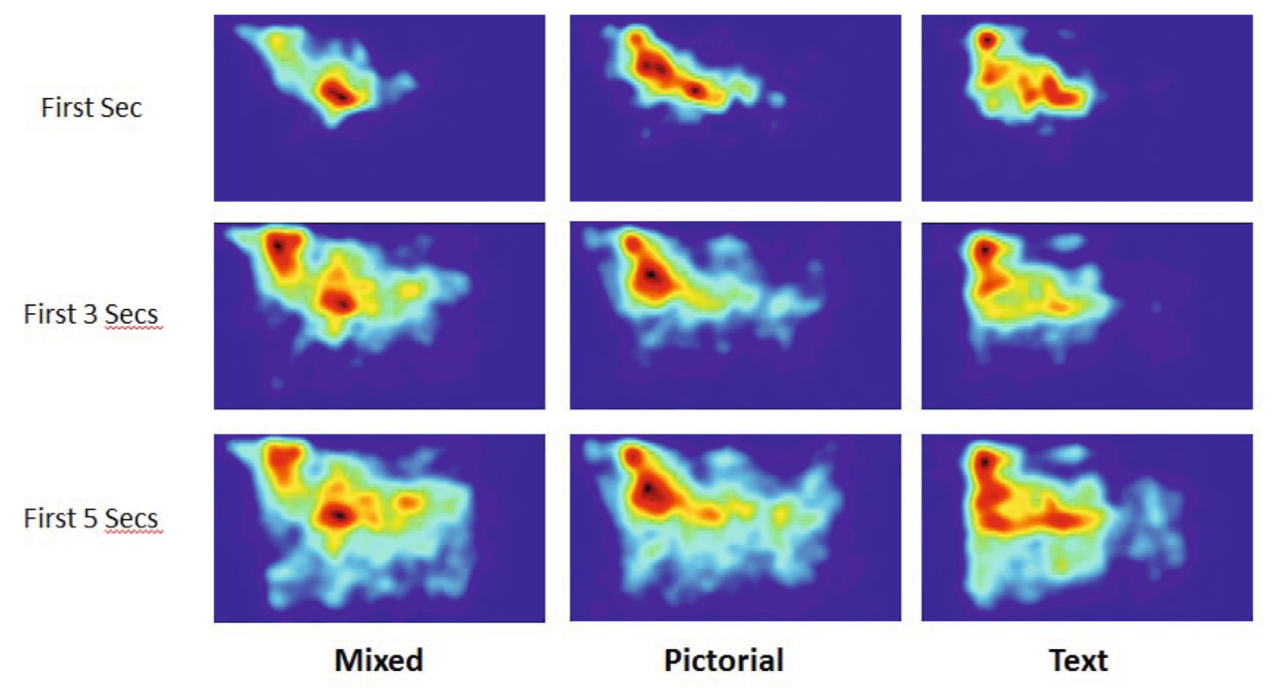
\includegraphics[width=8cm]{figures/shen-bias.png}
    \caption{Shenらのウェブページのヒートマップ生成実験結果\cite{shen2014webpage}}
    \label{fig_shen-experience}
\end{figure}

\par 本システムの位置情報による重み付けの手法をアルゴリズム\ref{alg:weight-position}に示す。要素の中心点の位置によって要素の顕著度の重み付けを行うことにした。左上の領域に大きな重みをつけるtop-left biasについては、横軸方向にどれだけの重みの差をつけるかを表すplace\_weight\_xと縦軸方向にどれだけの重みの差をつけるかを表すplace\_weight\_yの2つの数値を与える事で表現した。また、中心領域に大きな重みをつけるcenter biasにおいては中心部と最外部でどれだけ重みの差をつけるかを表すplace\_weight\_cを与える事で表現した。さらにtop-left biasとcenter biasを組み合わせる事で左上と中央部分に大きな重みをつけるf-biasを表現する。本研究においては横軸の重みの差を表すplace\_weight\_x = 0.1に縦軸の重みの差を表すplace\_weight\_y = 0.4に中心の重みの差を表すplace\_weight\_c = 0.2に設定した。正方形の20$\times$20マスのブロックをウェブページに見立てて重みの数値をシミュレーションした結果を図\ref{fig_fbias}に示す。左図はtop-left biasを、中央はcenter biasを、右図は2つを組み合わせたf-biasを表す。また、赤色に近くほど重みの数値が大きく白色に近くほど数値が小さいことを表す。さらに、図\ref{fig_fbias-test}にテスト用の同じ色の正方形を等間隔で並べたウェブページを入力した時の結果を示す。重み付け前の顕著性マップでは全ての正方形が同じ明度で表わされているが、重み付け後の顕著性マップでは左上から中央にかけての正方形の明度が高く表わされている事が確認できる。なお、認識しやすいように重み付け後の顕著性マップには顕著度のランキングを緑色の枠線の色で表している。

\par 最後に、要素毎に以上の重み付け処理を行なった結果の顕著度を最終的な出力に使用する為にCSVファイルに追記する。

\begin{algorithm}[H]
    \caption{位置情報による重み付け(F-bias)}
    \label{alg:weight-position}
    \begin{algorithmic}
    \Function{calc\_salient\_level}{start\_x, start\_y, size\_w, size\_h}
    \State salient\_level $ \leftarrow $ 要素の明度の平均値(0-255)
    \State width $ \leftarrow $ 顕著性マップの幅(px)
    \State height $ \leftarrow $ 顕著性マップの高さ(px) 
    \State place\_weight\_x $ \leftarrow $ 0.1 //横軸方向の重み
    \State place\_weight\_y $ \leftarrow $ 0.4 //縦軸方向の重み
    \State place\_weight\_c $ \leftarrow $ 0.2 //中心方向の重み
    \If{$size\_w < width$ and $size\_h < height$}
        \State x\_bias $ \leftarrow $ 1-(place\_weight\_x-((width-(start\_x+$\frac{size\_w}{2}$))*$\frac{place\_weight\_x}{width}$))
        \State y\_bias $ \leftarrow $ 1-(place\_weight\_y-((height-(start\_y+$\frac{size\_h}{2}$))*$\frac{place\_weight\_y}{height}$))
        \State top\_left\_bias $ \leftarrow $ x\_bias * y\_bias
        \State center\_bias\_x $ \leftarrow $ $|\frac{width}{2}-(start\_x+\frac{size\_w}{2})|^2$
        \State center\_bias\_y $ \leftarrow $ $|\frac{height}{2}-(start\_y+\frac{size\_h}{2})|^2$
        \State center\_bias $ \leftarrow $ $\sqrt{center\_bias\_x + center\_bias\_y} $
        \State salient\_level $ \leftarrow $ salient\_level*(topleft\_bias - (place\_weight\_c * center\_bias))
    \EndIf
    \State \Return salient\_level
    \EndFunction
    \end{algorithmic}
\end{algorithm}

\begin{figure}[H]
    \centering
    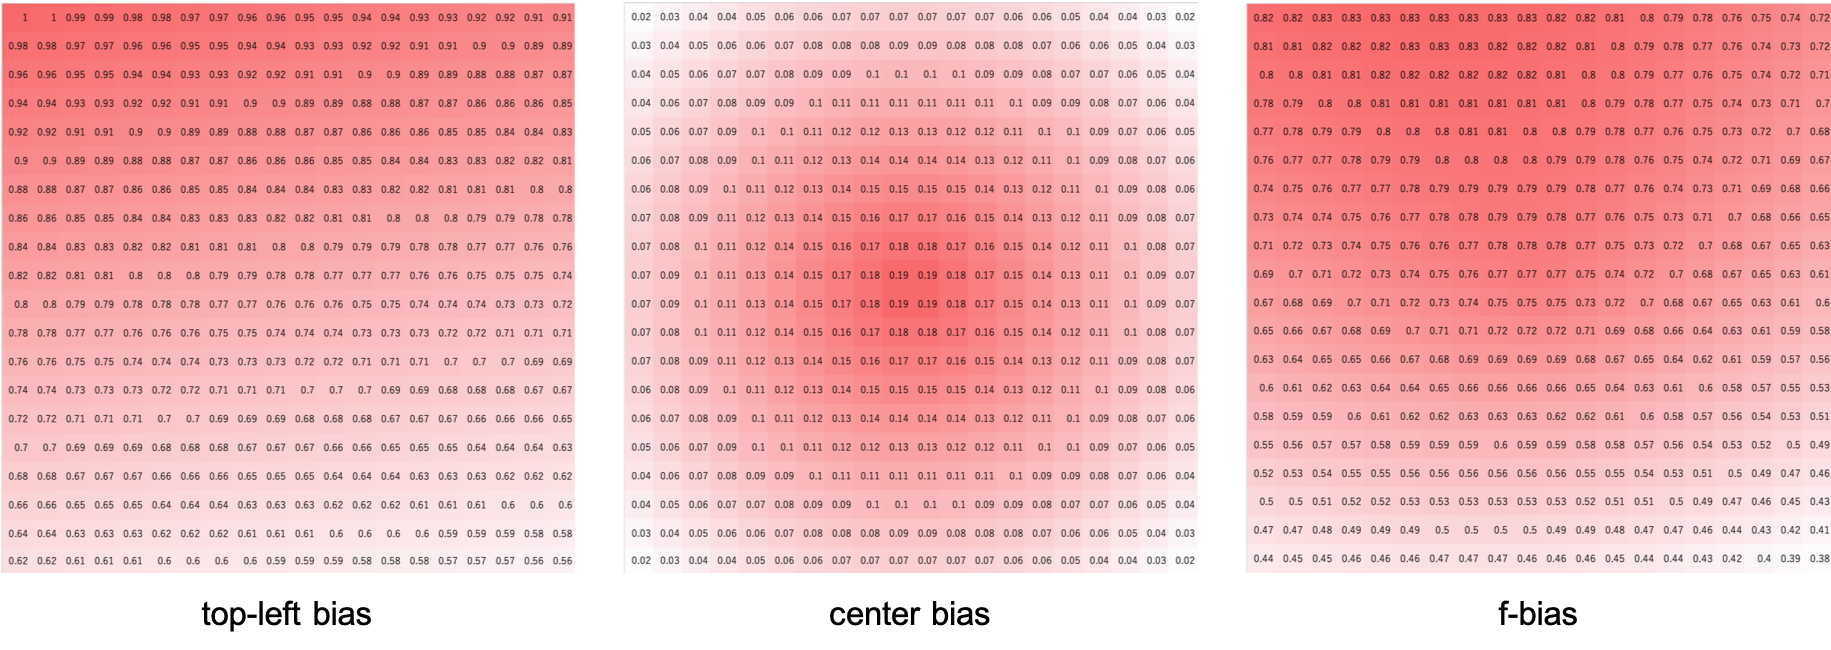
\includegraphics[width=12cm]{figures/fbias.png}
    \caption{位置情報による重み付けのシミュレーション}
    \label{fig_fbias}
\end{figure}

\begin{figure}[H]
    \centering
    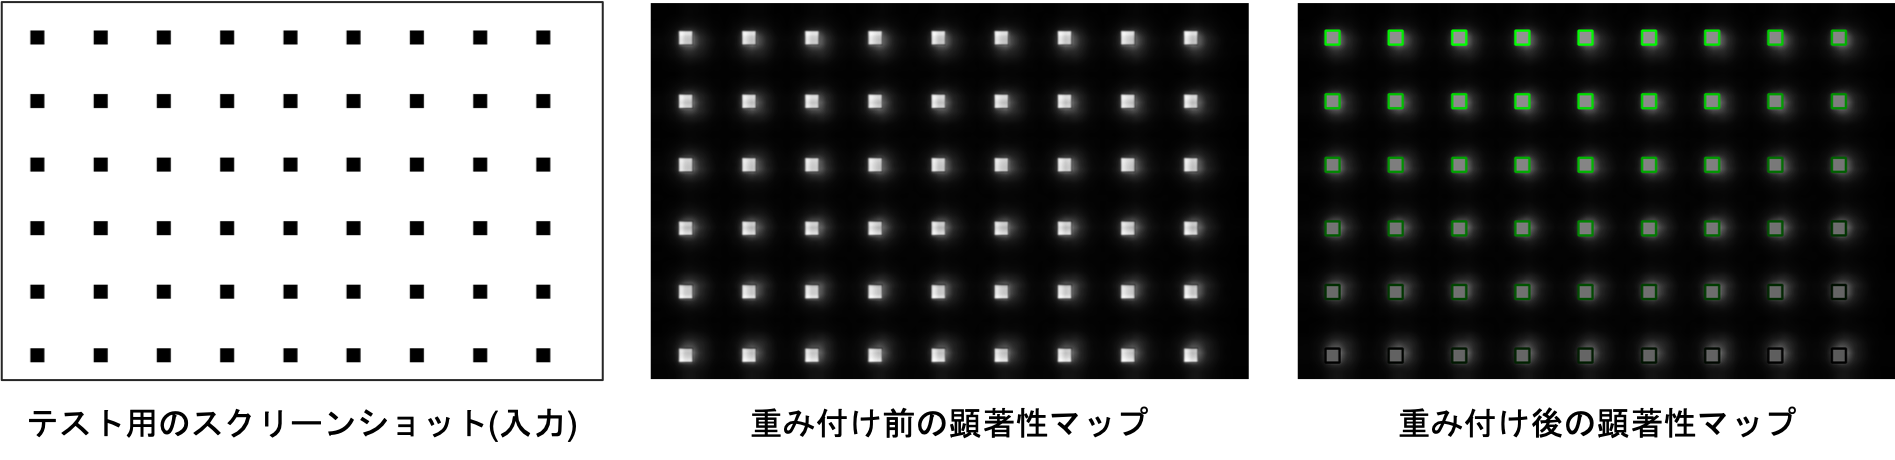
\includegraphics[width=12cm]{figures/fbias-test.png}
    \caption{テスト用ページを入力して得た顕著性マップ}
    \label{fig_fbias-test}
\end{figure}


\subsection{顕著領域の視覚化}\label{subsec:system04}
% 領域を塗りつぶして生成する顕著性マップと重要領域のランキングの生成方法の記述
\par ここでは第\ref{subsec:system03}節で計算した顕著度を元に顕著領域の視覚化を行う。本システムでは、顕著度が高い重要領域を要素単位で塗りつぶした顕著領域マップと特に顕著度が高い要素を一つにまとめた集約図の2つの出力を行う。顕著領域の視覚化の流れを図\ref{fig_system04}に示す。

\begin{figure}[H]
    \centering
    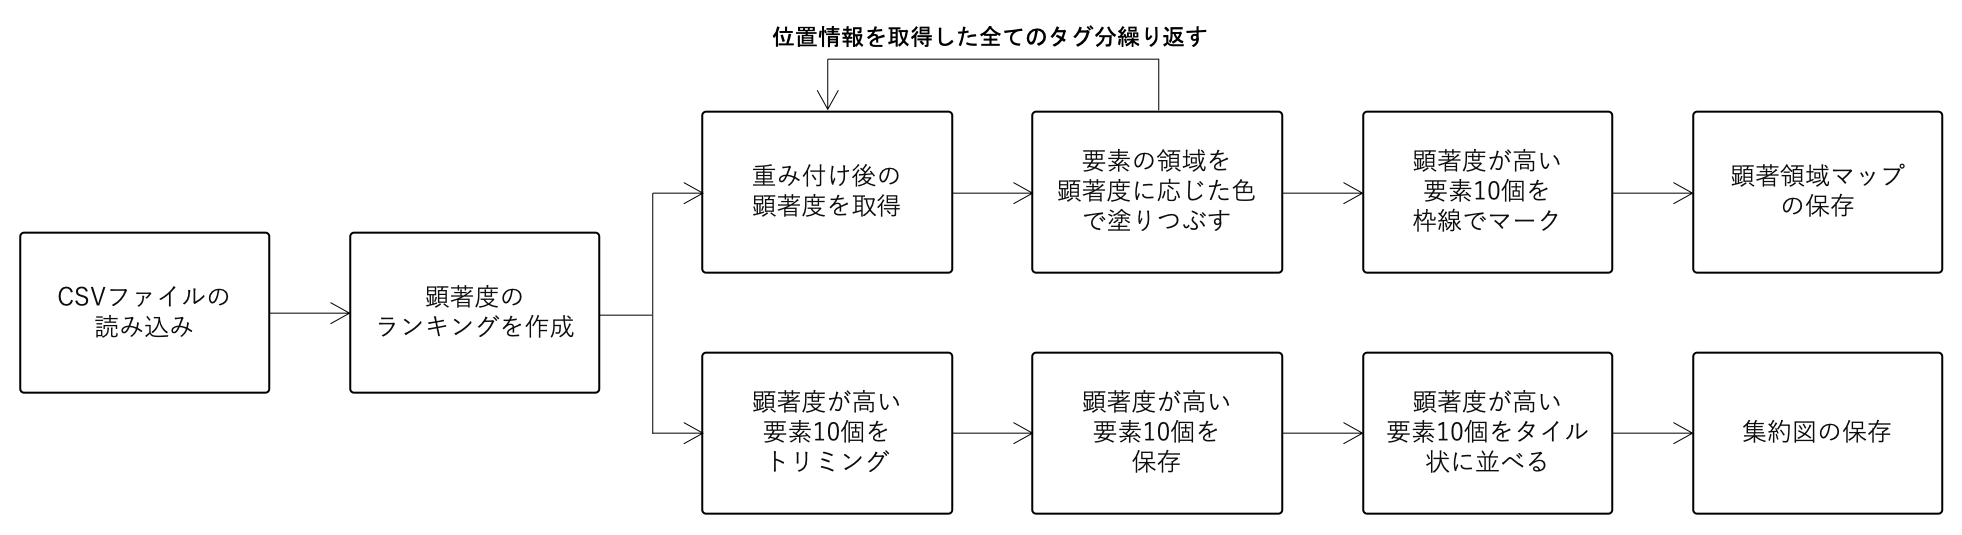
\includegraphics[width=12cm]{figures/system04.png}
    \caption{顕著領域の視覚化の流れ}
    \label{fig_system04}
\end{figure}

\subsubsection{顕著度ランキングの生成}\label{subsec:system04-1}
\par 顕著領域マップと集約図の生成にあたり、第\ref{subsec:system03}節で計算した顕著度のランキングを作成する。顕著度ランキングの計算アルゴリズムをアルゴリズム\ref{alg:lanking}に示す。まず始めに、第\ref{subsec:system03}節でCSVに保存した顕著度を顕著度が高い順にソートする。本来であれば、顕著度が高い順にランキングを付ければ良いが、図\ref{fig_system4-rank}に示すように同一要素を内包している他の要素も顕著度が高く評価されてしまう問題が生じる。同じ要素が顕著度ランキングに何度も出現する事は問題である為、一度顕著度が高いと評価した要素を内包する外部の要素をNGリストに格納して顕著度ランキングに入らないように評価する。



\newpage
\begin{algorithm}[H]
    \caption{顕著度ランキング}
    \label{alg:lanking}
    \begin{algorithmic}

    \State stag\_list $ \leftarrow $ CSVの読み組み, tag\_list\_num $ \leftarrow $ CSVの行数
    \State salient\_level = [] // 顕著度を格納するリスト, ng\_list = [] // NGリスト
    \State high\_element\_list = [] // 顕著度ランキングを格納するリスト
    \For{$i$ in $range(tag\_list\_num)$}
        \State salient\_level.append(tag\_listのi行目の要素の顕著度)
    \EndFor    
    \State salient\_level\_sort $ \leftarrow $ salient\_levelをソート
    \State salient\_num $ \leftarrow $ 10, temporal\_num $ \leftarrow $ 1, salient\_num\_first $ \leftarrow $ salient\_num

    \While{while salient\_num $>$ 0}
        \State most\_salient $ \leftarrow $ salient\_level\_sort[tag\_list\_num - temporal\_num]
        \If{(most\_salient in ng\_list) == False}
        \State start\_x, start\_y, end\_x, end\_y $\leftarrow$ CSVのmost\_salient行目から取得
        \State size $\leftarrow$ CSVからmost\_salient行目の要素のwidth $*$ heightを取得
        \If{(end\_x $-$ start\_x)/(end\_y $-$ start\_y) $<$ 10}
        \State high\_element\_list.append(most\_salient)
        \State salient\_num $\leftarrow$ salient\_num - 1
        \For{$i=1$ in $range(tag\_list\_num)$}
        \If{(most\_salient in ng\_list) == False}
        \State r\_start\_x, r\_start\_y, r\_end\_x, r\_end\_y $\leftarrow$ i行目から取得
        \State r\_size $\leftarrow$ CSVからi行目の要素のwidth*heightを取得
        \If{i行目要素とmost\_salient行目要素が内包関係}
        \If{r\_size $-$ size $<$ 200 $or$ size $-$ r\_size $<$ 200}
        \State ng\_list.append(i) //NGリストにi行目要素を格納
        \EndIf
        \EndIf
        \EndIf
        \EndFor 
        \EndIf
        \Else
        \State temporal\_num $\leftarrow$ temporal\_num $+$ 1
        \EndIf
    \EndWhile
    \end{algorithmic}
\end{algorithm}

\begin{figure}[H]
    \centering
    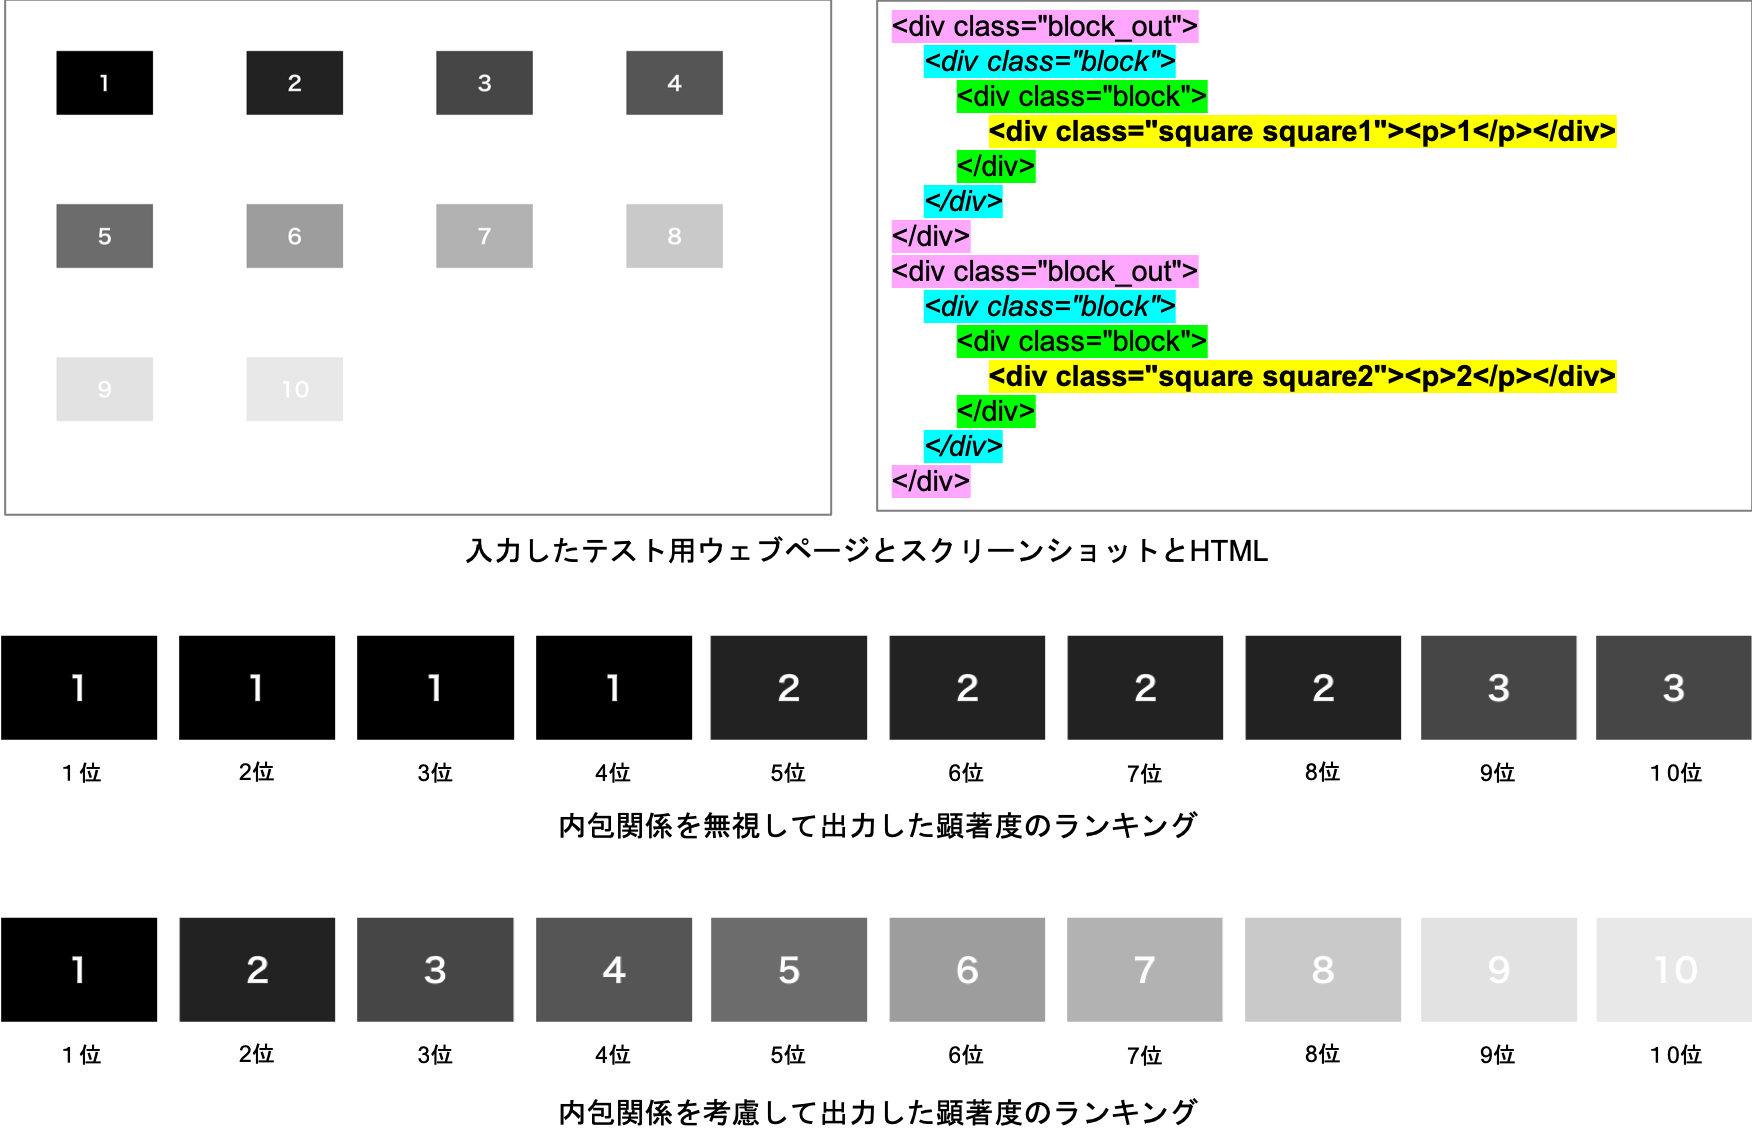
\includegraphics[width=12cm]{figures/include-rank.png}
    \caption{要素の内包関係を考慮した時としない時の顕著度ランキング}
    \label{fig_system4-rank}
\end{figure}

\subsubsection{顕著領域マップの生成}\label{subsec:system04-1}
\par 顕著領域マップの生成方法について説明する。第\ref{subsec:system03}節で計算した顕著度は0$\sim$255の範囲内の実数で表わされている。位置情報を取得した画面上に表示されている全ての要素の領域をこの顕著度を明度とした長方形で塗り潰す。また、第\ref{subsec:system03-1}節で説明した重み付けにより全体的に顕著度が低くなっている為、補正値を与える事ですべての要素の顕著度を補正値分高くすることとする。
\par さらに、特に顕著度が高い重要領域を視覚化する為に第\ref{subsec:system04-1}項で作成した顕著度ランキングの上位10個の要素の外枠を顕著度が高い順に明るい緑色の線で描写する。以上の作業を行う事で顕著領域マップの生成を行う。図\ref{fig_tile-example}に第\ref{subsec:system04-1}項で説明したテスト用ウェブページのURLを入力して生成された顕著領域マップの例を示す。

\subsubsection{集約図の生成}\label{subsec:system04-2}
\par 集約図の生成方法について説明する。第\ref{subsec:system04-1}項で作成した顕著度ランキングを元に顕著度が上位10個の要素の領域をスクリーンショットから切り取りタイル状に並べる。本システムでは上段に上位2個を、中段に3位$\sim$5位の3個を、下段には6位$\sim$10位の5個を並べる事で表現した。図\ref{fig_tile-example}に第\ref{subsec:system04-1}項で説明したテスト用ウェブページのURLを入力して生成された集約図の例を示す。


\begin{figure}[H]
    \centering
    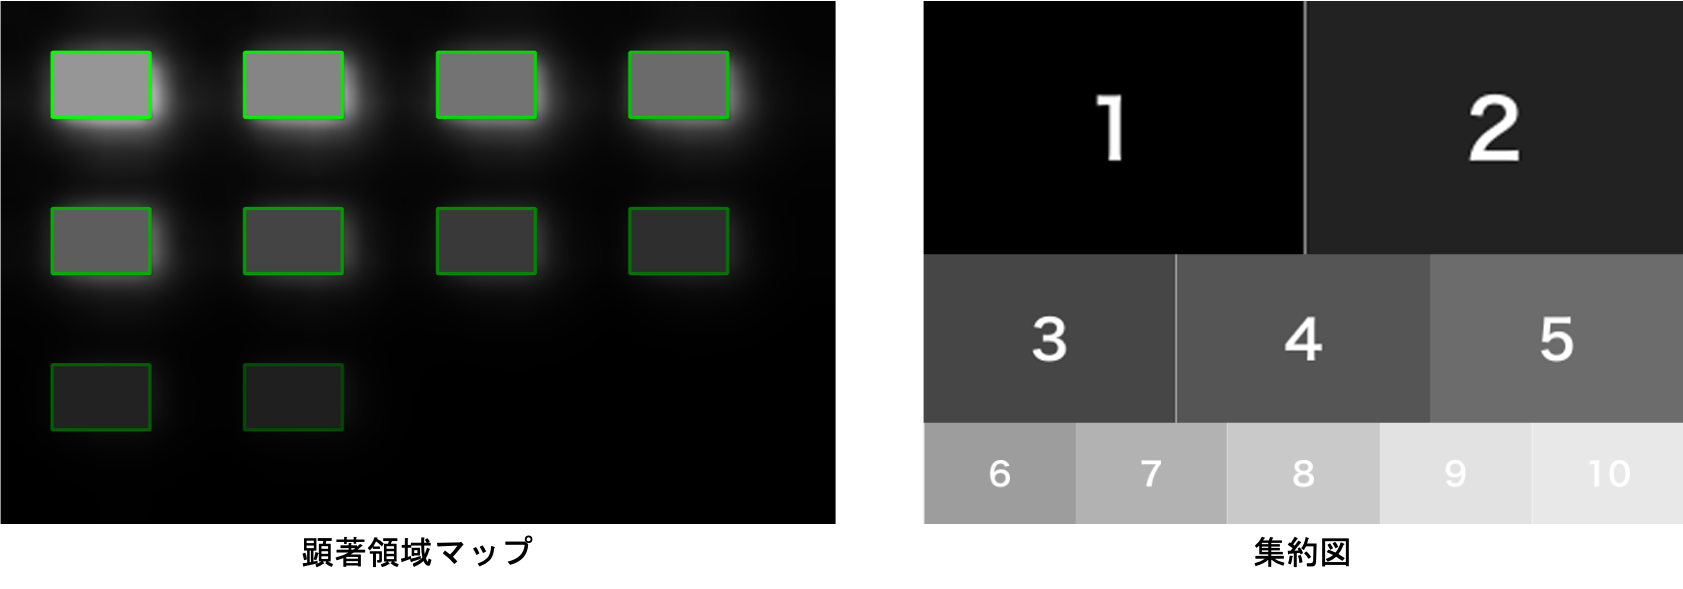
\includegraphics[width=10cm]{figures/example-output.png}
    \caption{生成される顕著領域マップと集約図の例}
    \label{fig_tile-example}
\end{figure}